\section{Introduction}
Introduzione agli argomenti trattati nel capitolo, dalle 4 alle 10 righe.

\section{\dots}
Argomenti trattati suddivisi sezione per sezione\dots

\section{Figure}
Per includere delle figure come la Figura~\ref{fig:figura} 
usare il comando \texttt{\\includegraphics}.

%--------------------------------------------------------------------------------
% esempio di inclusione immagine
%--------------------------------------------------------------------------------
\begin{figure}[tbh]
  \centering
  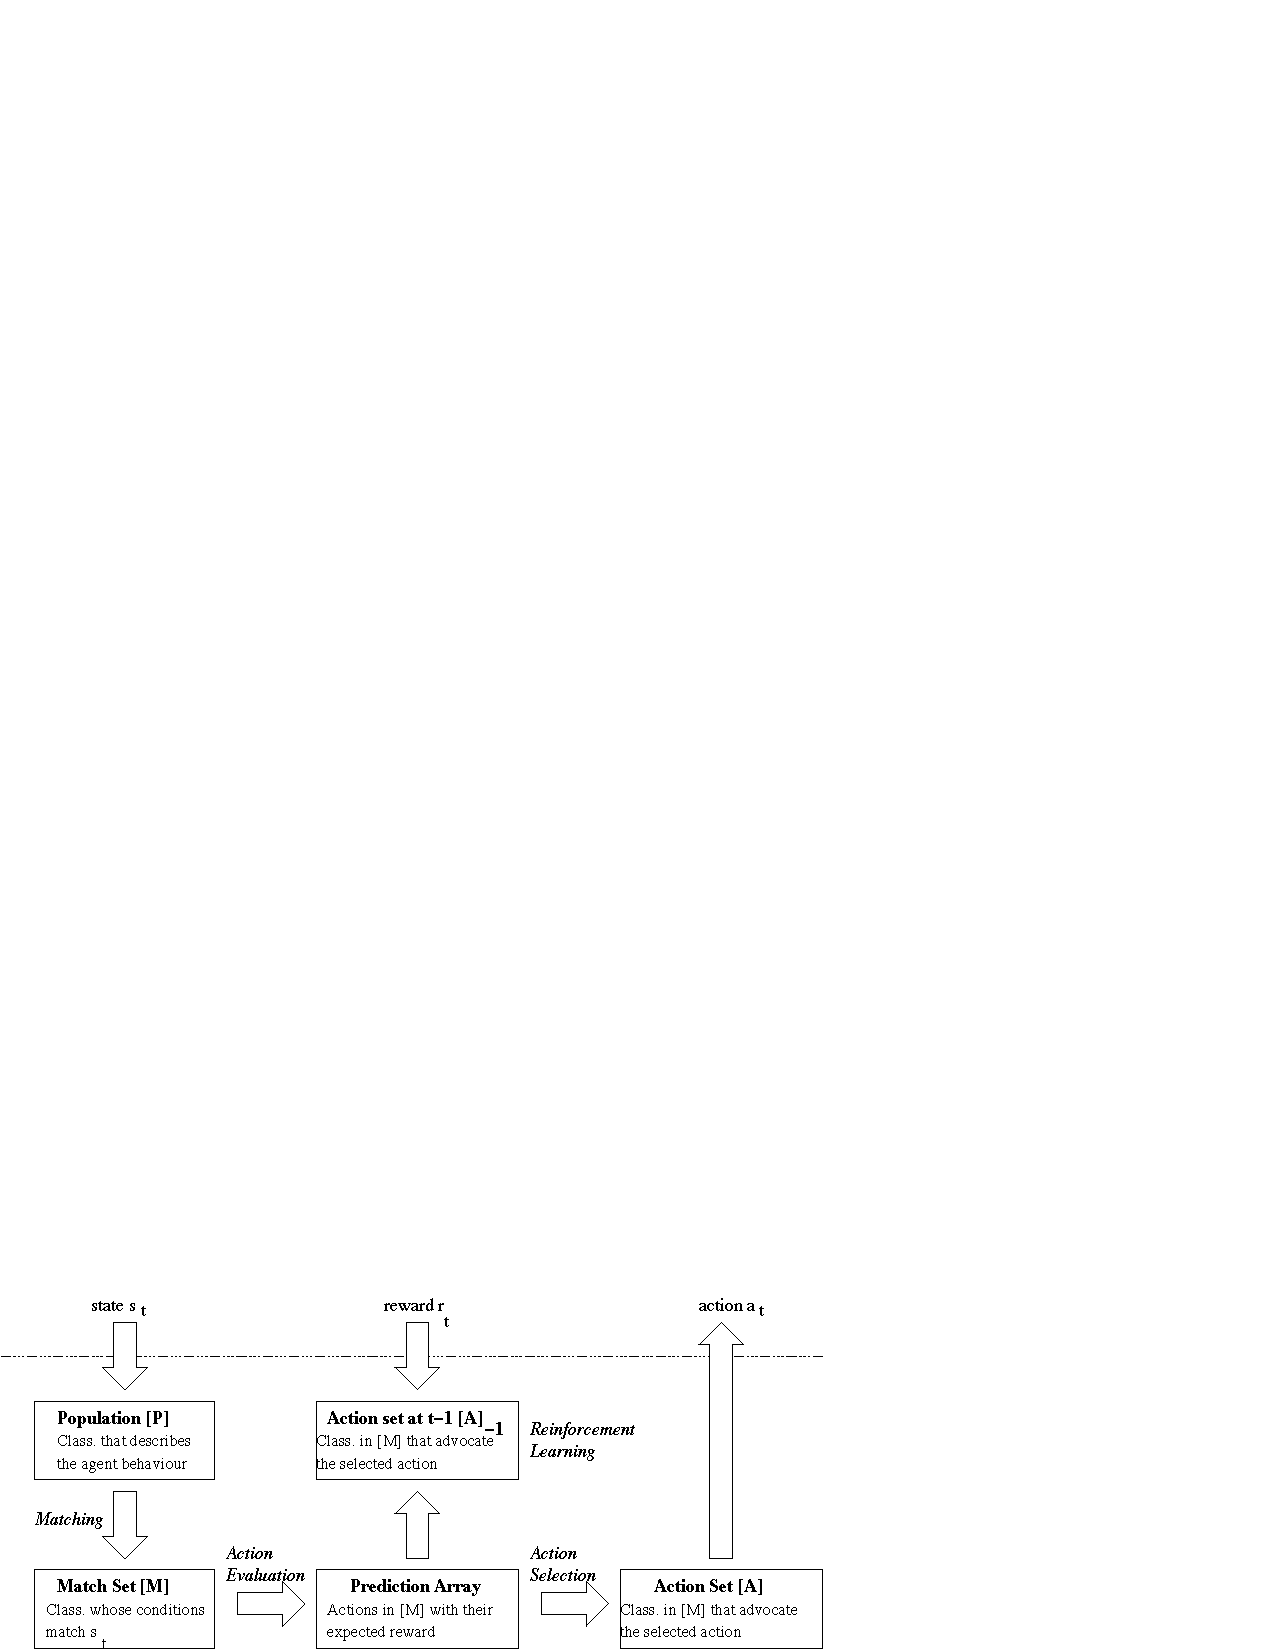
\includegraphics[scale=0.7]{images/esempio}
  \caption{\dots titolo}
  \label{fig:figura}
\end{figure}

\section{Algoritmi}
Per includere degli algoritmi come l'Algoritmo~\ref{alg:esempio}
usare lo stile \texttt{algpseudocode} presente nel package~\texttt{algorithmicx}.

%--------------------------------------------------------------------------------
% esempio di algoritmo
%--------------------------------------------------------------------------------
\begin{algorithm}[t]
  %%%
%%%
%%%	the Q-learning algorithm
%%%
%%%
\begin{algorithmic}[1]
\State Initialize $Q(\cdot,\cdot)$ arbitrarily
\ForAll{episodes}
   \State $t$ $\leftarrow$ 0
   \State Initialize $s_{t}$
   \Repeat
      \State $a_{t} \gets \pi(s_{t})$
      \State perform action $a_{t}$; observe $r_{t+1}$ and $s_{t+1}$
      \State $Q(s_{t},a_{t}) \gets Q(s_t,a_t) + \alpha( r_{t+1} + \gamma \max_{a\in A} Q(s_{t+1},a) -  Q(s_t,a_t))$
      \State $t \gets t+1$
   \Until{$s_{t}$ is terminal}
\EndFor
\end{algorithmic}

  \caption{Un esempio di algoritmo.}
  \label{alg:esempio}
\end{algorithm}


\section{Summary}

Riassunto del capitolo